%% ===================================================================
%%  DRAFT -- NOT SUBMITTED, NOT PEER REVIEWED.
%%
%%  Siting Atlas: a measurement paper.
%%  This file lives in a public repository BEFORE submission anywhere.
%%  Author and affiliation are deliberate placeholders.
%%
%%  Numbers policy: every figure in this paper is traceable to an
%%  artefact in the repository (outputs/metrics/*.json,
%%  outputs/tables/*.parquet, experiments/*/artefacts/*.json) or is
%%  re-derived from a committed data file, and is reconciled against
%%  docs/NUMBERS.md, which is the project's tie-breaker.  Where a
%%  quantity is NOT emitted by code into an artefact, the text says so
%%  at the point of use.
%%
%%  Build:  pdflatex siting_atlas_ieee.tex   (twice)
%%  No bibtex pass is required; the bibliography is inlined.
%%  refs.bib in this directory is the machine-readable twin and must be
%%  kept in sync by hand.
%% ===================================================================

\documentclass[conference]{IEEEtran}

\usepackage{graphicx}
\usepackage{url}
\usepackage{amsmath}

\graphicspath{{../docs/figures/}{../outputs/figures/}{./}}

\begin{document}

\title{What Open Data Cannot Tell You About Where\\a Warehouse Will Be Built:
A Pre-Registered Negative Result\\at Two Geographic Grains}

\author{\IEEEauthorblockN{[Author]}
\IEEEauthorblockA{[Institution]\\
\texttt{[email]}}}

\maketitle

\begin{center}
\fbox{\parbox{0.92\columnwidth}{\small\centering
\textbf{DRAFT --- NOT SUBMITTED, NOT PEER REVIEWED.}\\[2pt]
Published in a public repository before submission. Author and affiliation are
placeholders. Every figure is traceable to a repository artefact; where the
project's reconciliation document \texttt{docs/NUMBERS.md} disagrees with this
draft, that document is right.}}
\end{center}

\begin{abstract}
We report a pre-registered attempt to predict the siting of a single large
operator's last-mile delivery stations in the United States from free public
data, and its failure at both of the geographic grains we tested. The
hypothesis, sample, covariate list, baselines, evaluation metrics and numeric
success criterion were fixed and hashed before any model was fitted; the
resulting MD5 is recorded inside the result artefact and can be re-verified
against the sealed document. At metropolitan grain the fitted model beat a
zero-parameter ``rank metros by households'' baseline on out-of-time AUC in
\textbf{0 of 7} held-out years (pooled AUC 0.7323 against 0.8949; clustered
bootstrap difference $-0.1628$, percentile interval $[-0.2011, -0.1313]$ over
2{,}000 draws on 935 metro clusters), and was at least as well calibrated as a
constant null in only 3 of 7 years. At ZIP-code grain a conditional choice
model over 483 within-metro decisions is, on measurement, a single covariate:
on the 477-decision covariate-search frame, removing the count of warehousing
establishments drops large-metro top-10 lift from $6.22\times$ to
$2.68\times$, and ten of fifteen additional candidate covariates are bit-exact
no-ops. We give three supporting measurements. First,
a floor on the public-visibility gap: OSHA, the best free source of facility
locations, holds a record in only \textbf{138 of the 488} US cities where an
independent industry census lists a delivery station (28.3\%). Second, a
diagnosis with a screening rule: across 21 network terms in one run, low
within-metro dispersion is \emph{sufficient} for a covariate to fail (7 of 7
with coefficient of variation below 0.6 land on the parameter boundary) while
high dispersion is \emph{necessary but not sufficient} (9 of 14 above 1.3 are
interior), with the $0.6$--$1.3$ band empty. Third, a parcel-level cost model
--- a Daganzo-style continuous approximation whose depot layer is the
operator's \textbf{501 address-geocoded delivery stations} rather than a
solved network, covering 8{,}037 ZIP-code areas and 57.8\% of US households,
median \$1.1389 per parcel --- which does work, and which prices the
difference between real and optimal siting: substituting the observed
buildings for a 334-depot $p$-median raises the median \textbf{5.2\%} and more
than doubles median line haul, from 4.02 to 9.09 miles. Because cost falls as
$1/\sqrt{\delta}$, the cheapest places to serve are the densest and the
densest are where a warehouse cannot be built --- feasibility binds before
economics, which is also why a raw warehouse count out-predicts every
covariate we fitted. We also release a recovered
dataset of 1{,}904 facilities, 1{,}420 with opening years, OCR'd from an
industry document whose tables are images and validated three ways. The
contribution is methodological as much as empirical: pre-registration is rare
in applied siting work, and a registered null is a usable result.
\end{abstract}

\begin{IEEEkeywords}
pre-registration, negative results, facility location, discrete choice,
open data, last-mile logistics, data provenance, reproducibility
\end{IEEEkeywords}

% ===================================================================
\section{Introduction}
% ===================================================================

\IEEEPARstart{W}{here} a firm puts its next warehouse is a question with
public consequences --- traffic, air quality, tax abatements, local labour
markets --- and it is answered privately. A natural hope is that the growing
volume of free public data (census demographics, business patterns,
environmental screening layers, building permits) is enough to reconstruct the
decision from the outside, or at least to warn a community that it is on a
short list. This paper reports a sustained attempt to do that for one operator
and one facility class --- Amazon US small-package delivery stations --- and
reports that it does not work, at either of the two geographic grains we were
able to test.

The result is a null, and nulls are cheap to produce by accident. What makes
this one worth reading is the protocol around it. Before any metro-level model
was fitted we wrote and froze a pre-registration fixing the question, the
sample and its universe, the covariate list and the mechanism that motivated
it, both model families, three baselines, the evaluation design, five
conditions that would invalidate the test, and a numeric success criterion ---
together with the paragraph we would publish under each of the two possible
outcomes. The document was then hashed:

\begin{center}
\texttt{946f7ef75db69e5278eea409a04c3823}
\end{center}

\noindent That string is recorded in the result artefact's
\texttt{prereg\_md5} field, it is checked by continuous integration on every
push, and re-hashing the document today still reproduces it --- so a reader
does not have to take our word for the registration having been fixed in
advance; they can verify it in one command. Corrections discovered after the
fit were issued as a separate errata document rather than as edits, precisely
so that the seal would survive the corrections; one of those corrections runs
\emph{against} the registered hypothesis
(Section~\ref{sec:threats}).

\subsection*{Contributions}

\begin{enumerate}
\item \textbf{A pre-registered negative result at two geographic grains.}
The metro-entry model loses to ``rank by households'' on out-of-time AUC in 0
of 7 held-out years, under three model forms, in every size tercile, with and
without the 2020--21 pandemic build-out, and whether or not the model is
allowed to violate its own vintage rule. The ZIP-grain conditional choice model
is measurably one variable.

\item \textbf{A quantified public-visibility gap, reported as a floor.}
OSHA enforcement records --- the best free source of facility addresses ---
cover 138 of the 488 US cities in which an independent industry census lists a
delivery station.

\item \textbf{A diagnosis of why open data fails here that generalises beyond
this operator.} Most US public data is published at county grain or coarser. A
within-metro conditional choice model cannot use a variable that takes about
nine distinct values across two hundred candidate ZIP codes, however important
the underlying construct is. We tie this to an asymmetric dispersion
regularity and state its limits.

\item \textbf{A parcel-level cost model that does work, on an observed depot
layer.} The line-haul term is measured to the operator's 501 real
address-geocoded delivery stations rather than to a solved network, which both
removes the largest unclassified assumption in the model and prices it:
\textbf{+5.2\%} on the median and \textbf{$\times 2.26$} on median line haul.
The accompanying finding is that feasibility binds before economics --- the
cheapest ZIP codes to serve are the densest, and the densest are where a
warehouse cannot be built.

\item \textbf{A recovered dataset.} 1{,}904 facilities, 1{,}420 with opening
years, read out of an industry PDF whose tables are images, with three
independent validations run before any row entered a model.
\end{enumerate}

\subsection*{What this paper is not}

It is not a claim that Amazon's siting is unpredictable in principle, nor a
causal study of siting, nor a multi-operator generalisation. It is one
operator, one facility class, one panel, and a set of measurements about what
public data can and cannot support. Section~\ref{sec:threats} is the longest
non-results section in the paper for that reason.

% ===================================================================
\section{Related Work}
% ===================================================================

\textbf{No individual technique in this paper is novel.} Every component is a
standard method applied to a new dataset; the contribution is the measurement
and the protocol, not the machinery.

\emph{Facility location.} An earlier version of the depot layer solved a
$p$-median problem over candidate nodes; Hakimi's result that an absolute
median of a graph always lies at a vertex~\cite{hakimi1964} is what made a
discrete candidate set legitimate, and Klose and Drexl~\cite{klosedrexl2005}
survey the model family and its capacitated and multi-stage variants. That
solve is retired from the cost path. The depots are now observed, so the
relevant use of this literature here is as a \emph{benchmark}: the $p$-median
is the distance-minimising placement for a given number of sites, and the gap
between it and the operator's realised network is a quantity we report rather
than a modelling choice we make.

\emph{Continuous approximation.} The cost model computes distance per stop as
a line-haul term shared across a tour of $C$ stops plus a local term scaling
as $k/\sqrt{\delta}$ in stop density $\delta$. This structure is Daganzo's
\cite{daganzo1984ts}. \textbf{We must be explicit here: that paper has not
been read by the authors of this work.} It could not be obtained on the host
where the project was built; what was retrieved and read is its abstract
(via a bibliographic API), which confirms the object of the paper and, notably,
that zone \emph{shape} is its stated contribution --- something our
implementation does not represent at all. We therefore cite it for the
structure our code implements, and for nothing else. Related, and reported
here because it is a defect in our own bibliography that we found rather than
inherited: the second ``companion'' paper our code cited for the numeric
constant, DOI \texttt{10.1287/trsc.18.3.231}, is by
Vaughan~\cite{vaughan1984}, not Daganzo, spans pp.~231--244 rather than
231--253, and concerns average distances between random points in zones --- it
contains no tour, no vehicle and no tour-length constant, and supports nothing
in our cost model. A third 1984 Daganzo paper, on the length of tours in zones
of different shapes~\cite{daganzo1984trb}, is the more likely source of the
constant and was not cited by our code at all. The underlying limit theorem is
Beardwood, Halton and Hammersley~\cite{bhh1959}; the most accessible statement
of its constant is Larson and Odoni~\cite{larsonodoni1981}, \S6.4.8, which we
did read in full and which gives $K \approx 0.765$ --- 34\% above the $0.57$
our code uses. Section~\ref{sec:threats} states what we do and do not claim
about that gap.

\emph{Discrete choice.} The ZIP-grain model is a conditional logit over
within-metro choice sets, in the linear-in-attraction form. Train~\cite{train2009}
is the reference throughout, and specifically \S3.7.1 (printed p.~61) for the
independence-across-observations requirement that killed our survival model,
and \S3.4 Example~2 for the geographic-aggregation argument that motivates
entering covariates as extensive counts.

\emph{This operator.} Houde, Newberry and Seim~\cite{houde2023} estimate a
structural model of Amazon's fulfilment-centre network in \emph{Econometrica}
and are the closest prior work; several of our cost primitives are benchmarked
against their estimates, and they use the same industry facility census we OCR.
Holmes~\cite{holmes2011} is the methodological ancestor for economies of
density in retail network expansion.

\emph{Evaluation.} We report raw Brier scores and raw top-$k$ counts against a
uniform null and never a skill score, following Gneiting and
Raftery~\cite{gneiting2007} \S2.3 (p.~362), who show skill scores are
improper.

\emph{Data quality and linkage.} The facility panel is assembled by record
linkage across OSHA enforcement records, an industry census and a permit
trail. The formal model is Fellegi and Sunter~\cite{fellegisunter1969}; the
practical treatment we followed is Winkler~\cite{winkler1999rl}. The edit
system that accepts or rejects a row, and that supplies our validation rate, is
a Fellegi--Holt design~\cite{fellegiholt1976,winkler1999edit}. Rahm and
Do~\cite{rahmdo2000} supply the taxonomy of single- and multi-source problems
we used to structure the cleaning stage; Van den Broeck et
al.~\cite{vandenbroeck2005} the detect/diagnose/edit discipline.

To our knowledge there is no prior pre-registered study of private facility
siting from open data. That absence, rather than any technique here, is what
we think this paper occupies.

% ===================================================================
\section{Data}
% ===================================================================

\subsection{Recovering opening dates from an image-only document}

The binding constraint on any siting study of this operator is that nobody
publishes a dated facility list. MWPVL International, an industry consultancy,
publishes a network inventory --- the same source used by
Houde et al.~\cite{houde2023} --- but its tables are \emph{images}. All
thirteen were read by OCR. The extraction artefact
(\texttt{mwpvl\_extraction.json}, run \texttt{20260915-195231-c54f}) records:

\begin{center}
\begin{tabular}{lr}
\hline
Facilities extracted, 13 tables & 1{,}904 \\
\ldots with an opening year & 1{,}420 \\
\ldots with an opening month & 873 \\
\ldots flagged ``not confirmed'' by the publisher & 44 \\
US small-package delivery stations (eligible class) & 635 \\
\hline
\end{tabular}
\end{center}

The facts are MWPVL's; the contribution is reading them out of images and
testing them. Three independent validations were run \emph{before} any row
entered a panel.

\begin{enumerate}
\item \textbf{An OSHA cross-check} on all 1{,}420 dated rows. The edit
\texttt{E\_operating\_by} falsifies a stated opening date if an OSHA inspector
recorded the building as already operating before it. 208 rows linked to an
OSHA building, 11 were falsified: a \textbf{94.71\%} pass rate
(\texttt{mwpvl\_validation.json}, \texttt{20260915-195247-dbb5}). By stated
precision: month 160 matched / 9 falsified; year 25 / 2; quarter 23 / 0. The
same edit run against the 693-row assembled panel is a different denominator
and gives 95.59\% --- both are current and must not be conflated.

\item \textbf{Date plausibility}, 99.5\% $= (1{,}420 - 7)/1{,}420$: two dates
precede the start of the delivery-station network, five are beyond plausible.

\item \textbf{State agreement} between the OCR'd state column and the state
implied by the geocoded ZIP: 604 of 606 comparable rows agree, 99.67\%
(613 parsed of 635).
\end{enumerate}

The comparison that makes these numbers mean something is our own failed
satellite-dating programme, which produced an estimate for 107 of 107 sites
and then failed the \emph{first} of these tests on 36\% of its output: 39 of
107 estimates date construction \emph{after} the day an inspector found the
building already operating, a median of 33 months after. A 94.71\% pass rate
is not a certificate --- an unchecked row is not a passing row --- but it is
the difference between a method and a guess.

\subsection{The assembled panel}

\begin{center}
\begin{tabular}{lr}
\hline
Rows in the expanded facility panel & 693 \\
Buildings (rows surviving \texttt{E\_operating\_by}) & 687 \\
Distinct address+ZIP pairs & 691 \\
Rows with a numeric opening year & 551 \\
Distinct CBSAs / states & 230 / 50 \\
Latitude--longitude pairs in the panel CSV & 0 \\
\hline
\end{tabular}
\end{center}

The merge that produced it: 635 eligible rows in the extraction, 634 after
internal deduplication, 589 added as new panel rows, 40 already present, 5 held
for clerical review. A facility-class filter at the panel boundary excludes
1{,}269 rows of the wrong class; without it, fulfilment centres, Japanese
mini-stations and Canadian air hubs would have entered a US
delivery-station panel silently.

Three properties of this panel matter downstream and are stated here rather
than in a footnote. (i) The correct full sentence is \textbf{``483 decisions on
687 buildings from 693 rows''}; 691 distinct addresses is a fourth number and
is not ``buildings''. (ii) The panel carries \emph{no} coordinates, so every
distance covariate resolves to a ZCTA centroid; a side geocoding file reaches
72.3\% match (501 of 693) and is not joined in. (iii) 142 rows have a
non-numeric opening year and the panel deliberately fails its own numeric
check rather than dropping the rows or inventing a year.

\subsection{The visibility gap}
\label{sec:gap}

\begin{figure}[!t]
\centering
\includegraphics[width=\columnwidth]{fig_visibility_gap.png}
\caption{The public-visibility floor. Of the 488 US cities in which the MWPVL
industry census lists an Amazon delivery station, OSHA enforcement records ---
the best free source of facility addresses --- hold an inspection of any
Amazon facility class in 138; the other 350 are invisible to OSHA entirely.
Both counts are read at build time from
\texttt{outputs/metrics/mwpvl\_coverage.json}.}
\label{fig:gap}
\end{figure}

\begin{table}[!t]
\caption{The visibility gap, as counted. Two independent city lists, not a
numerator and a denominator. Source:
\texttt{outputs/metrics/mwpvl\_coverage.json}.}
\label{tab:gap}
\centering
\begin{tabular}{lr}
\hline
Cities where MWPVL lists a delivery station & 488 \\
Cities where OSHA ever inspected \emph{any} Amazon class & 340 \\
In both lists & 138 \\
MWPVL cities OSHA has never inspected & 350 \\
Share of MWPVL cities OSHA has seen & 28.3\% \\
\hline
\end{tabular}
\end{table}

The best free source of facility addresses in the US is OSHA enforcement data.
We measured how much of the network it sees, against the independent MWPVL
list (\texttt{mwpvl\_coverage.json}). Table~\ref{tab:gap} counts it and
Fig.~\ref{fig:gap} draws it.

These are \textbf{two independent city lists, not a numerator and a
denominator}. Two qualifications travel with the figure and we state them
every time it appears. It is \textbf{conservative}: OSHA's side is
unrestricted by facility class, so narrowing it to delivery stations would
widen the gap. And it is a \textbf{floor, not an estimate} --- a two-list
intersection, not capture--recapture --- because MWPVL is itself incomplete
and says so. A separate three-list capture--recapture exercise, using
OpenStreetMap as a third list whose capture mechanism is unrelated to worker
grievance so that dependence is \emph{measured rather than assumed}, puts OSHA
coverage of US cities with an Amazon facility at \emph{at most} 54.0\% under a
Chapman two-list estimator and at most 37.8\% under a Chao lower bound on the
population. Those are modelled estimates and a different quantity; the 28.3\%
is the thing that was counted.

\subsection{Covariates}

The choice model's frame joins households, land area, total establishments and
the County Business Patterns count of warehousing establishments, at ZCTA
grain, over 21{,}768 ZCTAs. Fifteen further candidates were tested, drawn from
the American Community Survey, EPA EJScreen and Census Building Permits
Survey. The relevant property of each is not its plausibility but its
\emph{within-metro variability}; Section~\ref{sec:disp} is about that.

% ===================================================================
\section{Methods}
% ===================================================================

\subsection{Within-metro conditional choice}

Conditional on one station opening in metro $m$, the probability that
candidate ZCTA $j$ is chosen is its share of the metro's total attraction,
$P_j = A_j / \sum_{k \in C_m} A_k$, with $A_j = \sum_c \beta_c x_{jc}$,
$\beta_c = \exp(\theta_c) > 0$, and $\beta_{\mathrm{households}}$ fixed at
1.0 as numeraire. Entering covariates as extensive counts in a linear
attraction is what makes the specification invariant to merging two ZCTAs
(Train~\cite{train2009} \S3.4, Example~2). Evaluation is by top-$k$ hit rate
against the analytic chance rate, \emph{stratified by choice-set size}, over
50 re-splits with the model refitted inside each repeat. Stratification is not
optional: in a metro with 25 or fewer candidates, random guessing already lands
in the top ten about two-thirds of the time, so pooled lift is capped by
arithmetic and pooling across strata is a Simpson's-paradox trap this project
fell into twice.

\subsection{The pre-registered metro-entry model}

Unit: CBSA $\times$ year, 2018--2025. Universe: all 935 CBSAs in the panel,
\emph{not} only the 195 that ever received a facility --- restricting to those
would be selection on the outcome and was named in advance as an invalidating
condition. Event: at least one delivery station opens in that CBSA in that
year. Both a logistic model on the binary event and Poisson / negative binomial
models on the count were fitted. Three baselines were fixed in advance:
(1) uniform, the no-information floor; (2) \textbf{rank by households}, named
in the registration as ``the one that matters''; (3) rank by facilities already
present, the densification null.

Primary evaluation is out-of-time: fit through year $t-1$, predict year $t$,
rolled forward. The registered success criterion is explicitly two-clause:
H1 is supported only if the model beats the households baseline on AUC in a
majority of held-out years \textbf{and} its calibration is at least as good as
a constant null in a majority of years. The second clause is where our earlier
survival model died, and the registration says why: ``ranking without
calibration is not prediction''.

Three arms were declared before any fit. \texttt{prereg\_strict} enforces a
strict vintage gate plus a 90\% per-year coverage floor and \emph{carries the
verdict}; \texttt{vintage\_clean} waives the coverage floor;
\texttt{vintage\_relaxed} ignores vintage entirely and is diagnostic only.

\subsection{Cost to serve}

For each ZCTA, daily parcels are derived from households and an
income-elasticity adjustment; stops from parcels per stop; stop density from
land area. Distance per stop is
\begin{equation}
\frac{d}{\text{stop}} \;=\;
\underbrace{\frac{k}{\sqrt{\delta}}\,\rho}_{\text{local}}
\;+\;
\underbrace{\frac{2L}{C}}_{\text{line haul}}
\end{equation}
with $\delta$ stop density per square mile of land, $\rho$ a circuity factor,
$L$ great-circle miles to the nearest depot and $C$ stops per tour. Cost per
stop is then a per-mile term, a per-hour driver term at 22\,mph, a flat
service time and a vehicle lease share. Five parameter scenarios are run end
to end.

\textbf{The depots are observed, not solved.} $L$ is measured to the nearest
of the operator's \textbf{501 address-geocoded delivery stations}. The
facility panel holds 693 rows; 192 carry only a ZCTA-centroid fallback
coordinate and are excluded, because a centroid depot sits inside its own
catchment by construction and drives that ZCTA's line haul to zero --- the
single most cost-reducing error available in this model. A ZCTA is costed if
its internal point lies within a 15-mile great-circle catchment of some
station; the catchment radius is the one this project pre-registered for an
unrelated analysis, so reusing it spends no new researcher degree of freedom.
Great-circle miles decide the catchment; the miles the model \emph{charges}
pass through $\rho$ exactly as the local term does.

The catchment is a trade of coverage against the regime the approximation is
valid in, and it is \emph{not} chosen for density. A sweep from 5 to 45 miles
is monotone in both directions: 5 miles gives a median 588 stops/sq.\,mi but
reaches 21.9\% of US households; 45 miles reaches 81.6\% at 44 stops/sq.\,mi.
\textbf{No radius is simultaneously denser than the retired pilot
(475 stops/sq.\,mi) and covers a majority of US households.} At 15 miles the
costed set is \emph{sparser} than the pilot --- 350 against 475 stops/sq.\,mi,
866 against 1{,}075 households/sq.\,mi --- and we report the resulting regime
violations rather than absorbing them (Section~\ref{sec:threats}).

Three coverage facts travel with every cost figure in this paper. Twenty of
the 501 stations contribute no costed ZCTA. Three hundred and sixteen ZCTAs,
0.83\% of catchment households, are dropped for carrying no OEWS driver wage
and \textbf{nothing is imputed}. Eight of the 501 stations are announced
rather than open.

\subsection{Reporting discipline}

Three rules are enforced throughout and are worth stating because they change
what the numbers mean.

\begin{enumerate}
\item \textbf{A percentile spread across re-splits is not a confidence
interval and not a standard error.} Every bracket we report from
\texttt{panel\_experiments}, \texttt{gravity\_network},
\texttt{metro\_entry} and \texttt{refit\_expanded} is a percentile over
re-splits of one fixed decision set; the artefacts carry an explicit
\texttt{spread\_is\_not\_a\_standard\_error} field. Only the metro-clustered
bootstrap intervals in this paper are bootstrap intervals.
\item \textbf{Raw scores, never skill scores}~\cite{gneiting2007}.
\item \textbf{Cite the artefact, not the figure.} Several headline numbers in
this project were invalidated by re-running the code that produced them, and
not one of those moves was caused by a parameter change.
\end{enumerate}

% ===================================================================
\section{Results}
% ===================================================================

\subsection{The metro-entry model: H0}

\begin{figure}[!t]
\centering
\includegraphics[width=\columnwidth]{fig_metro_auc.png}
\caption{The pre-registered result, drawn. Out-of-time AUC by held-out year
for the verdict arm (\texttt{prereg\_strict}, logit) against baseline~2, the
zero-parameter rule that ranks metros by household count. The model is the
lower line in all seven years and the pale bars are the yearly deficit. Every
value is read at build time from
\texttt{outputs/metrics/metro\_entry.json}.}
\label{fig:auc}
\end{figure}

\begin{table}[!t]
\caption{Out-of-time AUC by held-out year, verdict arm
(\texttt{prereg\_strict}, logit). 935 metros per year; 306 event metro-years.
Source: \texttt{metro\_entry.json}, run \texttt{20260915-231322-7d21}.}
\label{tab:metro}
\centering
\begin{tabular}{lrrrrr}
\hline
Year & Events & Model & B1 unif. & B2 h'holds & B3 fac. \\
\hline
2019 & 23 & 0.7487 & 0.5 & \textbf{0.9464} & 0.7198 \\
2020 & 49 & 0.6968 & 0.5 & \textbf{0.9682} & 0.7600 \\
2021 & 53 & 0.8119 & 0.5 & \textbf{0.9239} & 0.7811 \\
2022 & 36 & 0.7509 & 0.5 & \textbf{0.8780} & 0.7012 \\
2023 & 31 & 0.7713 & 0.5 & \textbf{0.9049} & 0.7934 \\
2024 & 50 & 0.6307 & 0.5 & \textbf{0.8363} & 0.6968 \\
2025 & 64 & 0.6098 & 0.5 & \textbf{0.8543} & 0.6902 \\
\hline
\multicolumn{2}{l}{pooled (6{,}545 rows)} & 0.7323 & --- & 0.8949 & 0.7325 \\
\hline
\end{tabular}
\end{table}

Table~\ref{tab:metro} is the result and Fig.~\ref{fig:auc} is the same seven
years drawn. Clause 1 of the registered criterion
fails \textbf{0 of 7}; the smallest yearly deficit is 0.112 of AUC (2021) and
the largest 0.271 (2020). Clause 2 fails 3 of 7. The verdict is \textbf{H0} on
every arm $\times$ form (three arms $\times$ logit / Poisson / negative
binomial, which agree to within 0.0001 of AUC in every year), and H0 also when
2020--21 are excluded, where it gets slightly worse (0 of 5 and 1 of 5).

We report the pre-registered H0 paragraph without softening, as written before
the fit:

\begin{quote}
\emph{Free public data cannot predict siting at any grain tested. The
ZIP-level failure is not a resolution problem but a general one: the variables
that drive the decision are not public at any resolution.}
\end{quote}

Four details sharpen this.

\emph{The fitted model reproduces a column of integers.} Pooled over the seven
held-out years, a two-covariate logistic fitted seven times scores AUC 0.7323;
baseline 3, the zero-parameter count of facilities already present, scores
0.7325 on the same 6{,}545 rows. Top-50 totals are 129 against 127.

\emph{Stratification strengthens the finding.} Terciles of households, fixed
across years: model AUC 0.4125 / 0.5666 / 0.6961 against baseline-2 AUC
0.7668 / 0.6827 / 0.8023, on 6 / 27 / 273 events. \textbf{The pooled AUC of
0.7323 is higher than the model's AUC in every single tier} --- the textbook
aggregation effect, since size both predicts the outcome and defines the
strata. Quoted alone, 0.73 would have read as a working model. Note also that
in the smallest tercile the model scores \textbf{0.4125, which is below the
0.5 of a coin flip}: on the six events among the smallest third of metros it
is not merely uninformative but actively mis-ordered. Six events is far too
few to make anything of that number on its own, and we make nothing of it ---
but it is the opposite of what a model that had learned a weak signal would
look like, and reporting the pooled figure alone would have concealed it.

\emph{The uncertainty is not marginal.} Metro-clustered bootstrap, 2{,}000
draws over 935 CBSA clusters: model AUC $0.7319\,[0.6876, 0.7706]$;
model minus households $-0.1628\,[-0.2011, -0.1313]$.

\emph{Leakage is not what is holding the model up.} The diagnostic
\texttt{vintage\_relaxed} arm --- seven covariates including households
itself, permitted to see data published after the year it predicts --- still
loses to ranking on households alone in 6 of 7 years, its single win being
$+0.0004$ of AUC, and loses calibration 7 of 7. \textbf{The ceiling is the
baseline.}

The single largest qualification on this run also belongs here, not in a
footnote. The registered vintage rule removed \textbf{8 of the 12
pre-registered covariates}, and two more failed the coverage floor, leaving
two. The reason is structural: most of the panel's columns are not time series
at all. Mean distinct values per unit across 32 quarters is exactly 1.00 for
population, households, income, the two EJScreen columns, both wage series and
metro employment --- one value, broadcast. The ACS 5-year 2023 file is built
from responses collected 2019--2023, so using it to predict 2020 is not a
borderline publication-lag call. \textbf{The Tier-1 mechanism that generated
H1 was therefore never testable on this panel.} That is a finding about data
availability rather than about the hypothesis, and it points at the same
conclusion from a different direction: the covariates that might have
distinguished one metro from another are published once, late, and without a
usable history.

\subsection{ZIP grain: the model is one variable}

On the \texttt{combined} arm (483 decisions, 258 in large metros, 193 held out
per re-split), the conditional logit's large-metro top-10 lift is
$6.2585\times$ over chance. Quintupling the panel from 94 to 483 decisions
bought no ranking accuracy and cost none: the same quantity is $6.1804\times$
on \texttt{original\_only} (94 decisions) and $6.2903\times$ on
\texttt{combined\_plus\_network}
(\texttt{panel\_experiments.json}).\footnote{Four different artefacts in this
project publish a ``large-metro top-10 lift'' on four different frames, with
different nulls and different numbers of splits. We name arm, method and
artefact every time.}

On \texttt{covariate\_search.json}'s frame (477 decisions, 191 held out,
687 facilities, run \texttt{20260915-235210-ff92}) the baseline is
$6.2157\times$ and the same model \emph{without}
\texttt{warehousing\_establishments} is $2.6785\times$. Removing one column
costs 3.54 of 6.22.

Of the fifteen additional covariates tested, \textbf{ten were exact no-ops} ---
the model was bit-identical with and without them on all 50 re-splits --- and
the best of the fifteen bought $+0.0082$ of lift. Two of the fifteen were
never independent tests: \texttt{vehicle\_availability\_total} is
\emph{equal} to \texttt{households} to floating-point precision on all 21{,}768
ZCTAs (both are ACS occupied housing units), and
\texttt{owner\_occupied} $+$ \texttt{renter\_occupied} $=$
\texttt{households} exactly, so those two rows are one test reported twice.
The corrected count is thirteen independent candidates.

\emph{Is the ceiling the data or the functional form?} A gradient-boosted
benchmark answers it. On the 94-decision frame, 38 held out, 50 repeats
(\texttt{gbm\_benchmark.json}, \texttt{20260915-200312-1d51}), quoting
\texttt{across\_repeats} because the artefact carries its own warning that a
$10^{-12}$ perturbation moves the single-split result by up to 2 of 38:
shallow GBM 22.26 hits, an unfitted raw warehouse count 20.96, the conditional
logit 20.60 (with the \emph{best} Brier of all methods, 0.007550), deep GBM
18.76. The flexible learner wins by about 1.3 decisions in 38 and loses on
probability quality; 53.5\% of its split gain sits on the one covariate.
\textbf{The ceiling is the data.}

\emph{Does the one working covariate contain its own outcome?} The count of
warehousing establishments is measured at a CBP vintage chosen off the
facility's OSHA-bounded opening year, which can post-date the building. A
decisive test forced the vintage behind the facility's \emph{stated} opening
date instead, on the 29 decisions where both exist, all three arms restricted
to the same 29 (\texttt{leakage\_decisive.json}, 50 paired re-splits):
\texttt{osha\_bound} 9.24 hits of 12, \texttt{true\_date} 8.22,
\texttt{no\_covariate} 4.48. The covariate retains
$3.74/4.76 = \mathbf{79\%}$ of its measured value and still beats the floor on
50 of 50 splits. The per-establishment coefficient is unchanged to within
1.2\% once each arm's column mean is divided out, which is what agglomeration
looks like rather than what a contaminated regressor looks like. It does not
survive cleanly: the test cost 65 of 94 working decisions, the test set is 12
decisions, and the design cannot separate the leak from the staleness that
removing it introduces --- so $+1.02$ hits is an \emph{upper bound} on the
leak, not a measurement of it.

\subsection{The dispersion regularity, and its asymmetry}
\label{sec:disp}

\begin{figure}[!t]
\centering
\includegraphics[width=\columnwidth]{fig_dispersion.png}
\caption{Why a covariate fails, term by term. Each point is one of the 21
network terms in \texttt{gravity\_network.json}
(run \texttt{20260915-210603-b780}), placed by its mean within-metro
coefficient of variation and by whether its coefficient is interior or at the
boundary in the arm where it is fitted. Every term below cv 0.6 is at the
boundary; 9 of the 14 above cv 1.3 are interior; the shaded band holds
nothing at all. The hollow marker is \texttt{fulfilment\_proximity}, interior
in one arm and boundary-straddling in another.}
\label{fig:disp}
\end{figure}

\begin{table}[!t]
\caption{Within-metro dispersion against coefficient state, all 21 network
terms. Low dispersion is sufficient for failure, high dispersion is necessary
but not sufficient for success, and nothing was observed in between.
Interior/boundary is the re-split percentile rule of the arm in which each
term is fitted. Source: \texttt{gravity\_network.json}, run
\texttt{20260915-210603-b780}, \texttt{terms.dispersion} at vintage 2030.}
\label{tab:disp}
\centering
\begin{tabular}{lrrr}
\hline
cv band & terms & interior & not interior \\
\hline
$< 0.6$ & 7 & \textbf{0} & \textbf{7} \\
$0.6$--$1.3$ & 0 & --- & --- \\
$> 1.3$ & 14 & 9 & 5 \\
\hline
\end{tabular}
\end{table}

A conditional choice model differences away everything constant within a
choice set. A covariate's only currency is therefore how much it varies among
the $\sim$200 candidate ZCTAs of one metro. Measured directly, the mean number
of distinct values per large metro is 200 for land area and 193 for households,
but \textbf{9.2} for the EJScreen and ACS county-grain columns and 8.0/7.9 for
the two building-permit columns. Six of eighteen columns offer the model nine
distinct values with which to rank two hundred alternatives.

This can be turned into a pre-fitting screen. Over 21 network terms in one run
(\texttt{gravity\_network.json}, \texttt{20260915-210603-b780},
\texttt{terms.dispersion} at vintage 2030, 41 large metros of $\geq$101
candidates, 8{,}271 candidate ZCTAs), scoring each term's mean within-metro
coefficient of variation against its boundary/interior state in the arm where
it is fitted gives Table~\ref{tab:disp}. Fig.~\ref{fig:disp} plots the same 21
terms one by one rather than banded.

\textbf{The rule runs one way.} Low within-metro dispersion is
\emph{sufficient for failure}: all 7 terms with cv below 0.6 (range
0.2975--0.5918) land at the coefficient boundary. High dispersion is
\emph{necessary but not sufficient for success}: 9 of the 14 with cv above 1.3
(range 1.3993--8.5046) are interior, and the 5 that are not are all on the
sortation side, four of them carrying square footage as mass. An earlier
version of this claim, including the version quoted in our own
pre-registration, asserted the rule held ``21 of 21'' in \emph{both}
directions; it does not, and the two-way version was exactly the part that
made it sound like a predictor.

Two things raise this above coincidence in the direction it does run. The
gravity exponent $\alpha$ is a \emph{knob}: moving it from 1 to 3 changes
nothing about what the covariate measures --- still pull from the same
facilities --- and changes only how sharply it discriminates within a metro.
The cv rises from 0.30 to 8.50 and the coefficient walks from the boundary to
the interior. And it retrospectively explains the one failure that had no
explanation: a \emph{count} of facilities within 50 miles sits at cv 0.59 and
fails at 25, 50 and 100 miles, while a \emph{distance} to the same facilities
works. The radius was never the issue.

\textbf{Read this as description, not as an estimated relationship.} $n=21$
terms from a single run at a single vintage, and the terms are not independent
--- each is one of two columns in one of 13 arms fitted over the same 483
decisions. Nothing was observed between cv 0.6 and 1.3, so the finding is
silent about intermediate dispersion. We state it as a screening heuristic
worth seconds of compute before fitting anything, and no more than that.

\subsection{The cost model works, and says feasibility binds first}
\label{sec:cost}

\begin{figure}[!t]
\centering
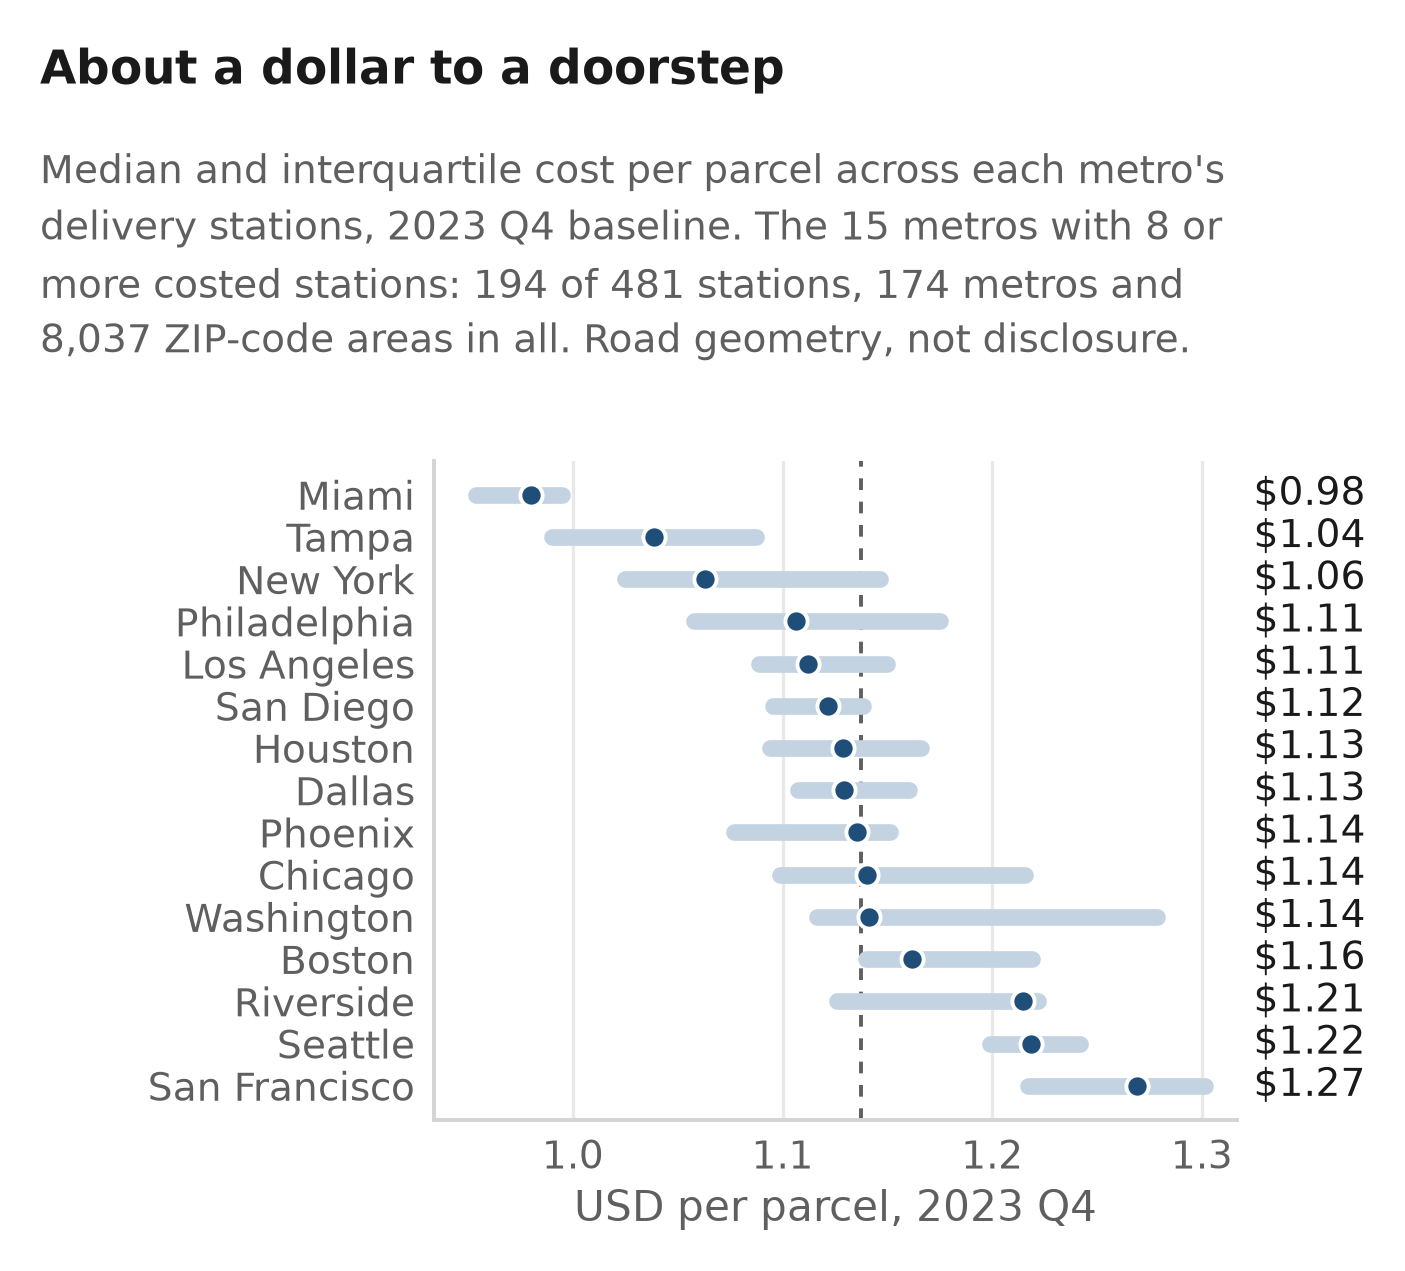
\includegraphics[width=\columnwidth]{fig_cost_by_metro.png}
\caption{Median and interquartile cost to deliver one parcel, by metro
(2023\,Q4 baseline scenario, observed depot layer). Every value is read at
build time from
\texttt{outputs/tables/cost\_by\_station\_2023q4\_baseline.parquet}; nothing
in the figure is typed by hand. The 15 metros drawn are those with at least
eight costed stations --- 194 of the 481 stations, selected by a threshold
rather than a rank because eight metros tie at five stations and a ``top
$n$'' cut would break that tie arbitrarily. The remaining 159 metros are
mostly single-station, where an interquartile bar has no content: the median
metro-level IQR across all 174 is \$0.00.}
\label{fig:cost}
\end{figure}

\begin{table}[!t]
\caption{The 2023\,Q4 baseline cost model on the observed depot layer, over
8{,}037 ZCTAs and 501 real delivery stations. Source:
\texttt{cost\_by\_station.json}, \texttt{run\_id 20260916-131845-34f1}; the
per-ZCTA and per-station tables it is computed from ship with the repository.}
\label{tab:cost}
\centering
\begin{tabular}{lr}
\hline
Median cost per parcel & \$1.1389 \\
p10 / p90 & \$1.0008 / \$1.3445 \\
Pooled cost per parcel & \$1.1281 \\
ZCTAs costed & 8{,}037 \\
Households covered & 74{,}399{,}605 (57.8\%) \\
Stations (real / with a costed ZCTA) & 501 / 481 \\
Metros containing a station & 174 \\
Median line haul & 9.09 mi \\
Total daily parcels & 42{,}048{,}849 \\
Total daily cost & \$47{,}434{,}701 \\
Vans ($\lceil \sum \text{van-days} \rceil$) & 250{,}291 \\
\hline
\end{tabular}
\end{table}

Table~\ref{tab:cost} summarises the baseline scenario and Fig.~\ref{fig:cost}
shows how it distributes across metros. Across the five parameter scenarios
the median moves from $-17.2\%$ (dense routing, \$0.9431) to $+7.7\%$
(congested, \$1.2264).

\begin{table}[!t]
\caption{What replacing a solved depot network with the observed one costs.
The pilot column is a Daganzo model identical in every parameter, differing
only in that its depots are a 334-site $p$-median over ten metros. Source:
\texttt{cost\_by\_station.json}, \texttt{pilot\_comparison}.}
\label{tab:depotswap}
\centering
\begin{tabular}{lrr}
\hline
& solved depots & observed depots \\
\hline
Depots & 334 $p$-median & 501 real (481 used) \\
ZCTAs costed & 2{,}333 & 8{,}037 \\
Median cost per parcel & \$1.0830 & \$1.1389 \\
p10 / p90 & 0.9778 / 1.4180 & 1.0008 / 1.3445 \\
Median line haul (mi) & 4.02 & 9.09 \\
Service time share & 66.96\% & 59.75\% \\
Vehicle share & 22.93\% & 21.63\% \\
Drive-time share & 6.97\% & 12.63\% \\
Distance share & 3.14\% & 5.98\% \\
Scenario span on median & $-17.1/+4.4\%$ & $-17.2/+7.7\%$ \\
\hline
\end{tabular}
\end{table}

\textbf{The level is the least interesting line in Table~\ref{tab:depotswap}.}
Replacing the solve with the observed network moves the median \textbf{+5.2\%},
which is inside the width of a single stress scenario. What moves materially is
the \emph{composition}. Median line haul more than doubles, 4.02 to 9.09 miles,
because a real national network is not a distance-minimising one --- and
because the costed universe is now national rather than ten dense metros. Drive
time and distance together rise from \textbf{10.1\%} of a stop to
\textbf{18.6\%}. Labour at the door still carries the bill at 59.75\%, but the
summary this project previously published --- that the routing mathematics is
decoration --- described the solved network and no longer holds. The
consequence for this paper is that the parameters now carrying the headline
have shifted from \texttt{service\_minutes\_per\_stop} toward
\texttt{avg\_speed\_mph}, \texttt{circuity} and \texttt{van\_mpg}, none of
which has an external source (Section~\ref{sec:threats}).

\textbf{A $p$-median is a lower bound, so the 5.2\% is a measurement.} The
solve minimises demand-weighted distance by construction; the operator's
buildings sit where land, labour, zoning and lease terms allowed. The gap
between the two is the cost of siting in the world rather than in the
objective function, and on this network it is 5.2\% of the median parcel and a
doubling of line haul. We know of no comparable figure computed on a real
US last-mile network from public data.

\textbf{Feasibility binds before economics, and this is an argument about the
cost function rather than a statistic.} Cost falls as $1/\sqrt{\delta}$. The
cheapest ZIPs to serve are therefore the densest, and the densest are
precisely where a warehouse cannot physically be built --- no parcel, no dock,
no zoning, no lease. That is also why a raw warehouse count out-predicts
everything else we fitted: the count measures where building is
\emph{possible}, not where delivering is cheap.

\textbf{A statistic supporting that claim is withdrawn, and the withdrawal is
itself a result.} Earlier versions of this work reported that of 43 pilot
facilities, zero sat in the cheapest decile of their own metro. That test is
\textbf{not identified on the present model} and we do not restate it with new
digits. Once the depots \emph{are} the facilities, a ZCTA containing a station
has a line haul of approximately zero because the station is inside it; line
haul enters as $2L/C$ and drive-plus-distance is 18.6\% of the bill, so the
model makes every facility's own ZCTA cheap by construction. Ranked on the
published frame, 275 of 476 matched facilities (57.8\%) land in the cheapest
decile at a median percentile rank of 0.080 --- the circularity, measured.
Re-pricing every ZCTA against the nearest station \emph{outside} it does not
rescue the test: the mask gives \textbf{33 of 476 (6.9\%)} for the 501
stations but \textbf{7 of 43 (16.3\%)} for the original pilot facilities,
below and above the 10\% a uniform placement would give. The mask
under-corrects in dense metros, where a masked station's neighbour is two
miles away (median masked line haul 6.8 miles for the 43 against 10.4 for the
501). A statistic whose sign depends on which facility set draws the
counterfactual is not evidence for either sign. The mechanism in the preceding
paragraph does not depend on it.

\subsection{Three further programmes, each retired on a measurement}

\emph{Survival.} A ZIP-quarter hazard model was rebuilt on $6.7\times$ the
events (812 $\rightarrow$ 5{,}441) with real recovered opening dates. AUC held
out by unit moved 0.6894 $\rightarrow$ 0.6832, and a constant null was better
calibrated in \textbf{17 of 17} comparisons
(\texttt{hazard\_revival.json}; \texttt{model\_better\_calibrated\_at} is an
empty list). The retirement was taken on the unit of analysis, not sample size:
one opening switches on a \textbf{median of 39 ZCTAs} at the 15-mile catchment
(mean 52.4, max 317), which the likelihood counts as 39 independent
observations. No radius between 8.3 and 45 miles brings that below 14.

\emph{White space.} Ranking unserved places by an under-coverage score wins
\textbf{14 of 108} scored cells (13\%), with \textbf{0} significant wins for
white space against 32 for the household baseline. What it did produce is a
densification measurement: at the headline 45-mile radius, \textbf{68.7\%} to
\textbf{75.9\%} of 2024--25 delivery-station openings landed inside coverage
the pre-2024 network already had (75.9\% = 60 of 79 openings with real Census
coordinates; 68.7\% = 90 of 131 once ZCTA-centroid fallbacks are admitted).
That range is across \emph{coordinate sets at one radius}, not across radii.

\emph{Gravity.} Replacing distance-to-nearest with summed distance-discounted
network pull produces the only specification whose coefficients never hit the
boundary, and when both are offered the optimiser keeps gravity and discards
distance --- a better measurement. It does not resolve to a single scalar
against proximity: on large-metro top-10 lift the best fully-interior gravity
arm scores 6.2187 against the published proximity baseline's 6.2903 and a
no-network floor of 6.2585, but paired over the same 50 re-splits it is
$+0.0116$ on top-1 (42 improved / 4 worsened), $+0.0126$ on top-5 (44 / 2) and
$-0.0002$ on top-10 (18 / 22), and it wins on Brier. It also costs the
specification its aggregation argument: over 43{,}224 merged ZCTA pairs the
merger-invariance error is 0.00 for the extensive-only control and 0.044
median / 0.455 maximum for the network arm. We did not switch.

% ===================================================================
\section{Discussion}
% ===================================================================

\subsection{Why open data fails here, and where that generalises}

The two failures have one diagnosis and it is about publication grain, not
about the world.

A within-metro conditional choice model can only use a covariate that varies
\emph{inside} a metro and is \emph{not} a population proxy. Most free US
public data fails one or both. County-grain series --- environmental
screening, permits, wages --- are broadcast down to every ZCTA in the county
and arrive at the model as about nine distinct values across two hundred
alternatives. A constant cannot rank anything, however large its true effect.
This is not a data-quality problem: \texttt{traffic\_proximity} is populated on
99.9\% of rows. And the remaining ACS columns are collinear with the numeraire
by construction --- a ZCTA with twice the households has twice the cars, twice
the labour force, twice the graduates --- so they are not identified. When we
re-entered them as per-household rates the collinearity was repaired
(within-metro correlation with households falling from $+0.982$ to $+0.112$ for
labour force, from $+0.909$ to $-0.368$ for owner-occupancy) and the lift did
not move. The failures were over-determined: the columns were collinear
\emph{and} empty.

Escaping to metro grain was the obvious move, and it is the move the
pre-registration bet on: variation that is between counties is, by
construction, between metros. The bet lost, and the way it lost is the
interesting part. The county-grain covariates could not be used at metro grain
either --- not because they lack variation there, but because they are
published \emph{once, late, and without a usable history}, so no
time-respecting vintage of them exists. The transparency gap therefore has two
distinct components: variables published too coarsely to discriminate within a
market, and variables published without the temporal depth to predict anything
at all. Section~\ref{sec:gap}'s 138-of-488 is a third: the locations
themselves are largely unrecorded in public enforcement data.

\subsection{What would actually move this}

Our own evidence names the candidates, and they share a shape. The covariates
that work are the ones \emph{computed as a distance from each candidate}
rather than \emph{looked up against it} --- because the former are
ZCTA-specific by construction and the latter inherit the publisher's grain.
The two network-proximity terms are the only new class that ever worked. The
best untested idea by the same logic is parcel-level land data (acreage, zoning,
van-staging capacity): finer than ZIP and uncorrelated with population, it
passes both filters. It is blocked on roughly three thousand county GIS
portals, which is an infrastructure problem rather than a modelling one --- and
that is itself the paper's point.

\subsection{On pre-registration in applied siting work}

Writing the registration cost about a day and changed three decisions we would
otherwise have made after seeing results. It fixed the households baseline as
the bar \emph{before} we knew the model would clear only the uniform one; it
fixed the calibration clause \emph{before} we knew the model would rank
tolerably and calibrate badly; and it wrote the H0 paragraph in advance, which
is the main reason this paper reports a null in the language of a finding
rather than of an excuse. It also produced three criticisms of itself that only
became visible once it met the data --- most usefully, that its covariate list
should have been checked for distinct-values-per-unit before being fixed, a
two-line check. That is an argument for writing one, not against it.

% ===================================================================
\section{Threats to Validity}
\label{sec:threats}
% ===================================================================

\subsection{The panel is one operator, one class, one country}

Every result here is Amazon US small-package delivery stations. Nothing
licenses extrapolation to other operators, other facility classes or other
regulatory regimes. The visibility gap in particular depends on OSHA's
inspection selection, which is driven by worker grievance and is therefore not
independent of facility age, size or unionisation.

\subsection{The leakage test rests on 29 decisions}

The audit of the load-bearing covariate cost 65 of 94 working decisions (69\%)
and leaves a 12-decision test set, fitting 17 decisions against 3 estimable
parameters. Its intersection is also not a random subsample: \texttt{osha\_bound}
scores 77\% here against 54\% on the full 94, so these 29 buildings are
measurably easier. Fourteen of the 29 stated dates come from an MWPVL table for
a \emph{different} facility class matched on the same street address;
restricting to the two delivery-station tables halves the sample to 15
decisions, 6 held out, and the difference disappears into noise. Nothing was
corrected: two of the 29 stated dates are later than the OSHA bound for the
same building, and are used as stated, because dropping the pairs that
disagree in the inconvenient direction is how a leakage test is rigged.

\subsection{The dispersion finding is descriptive and from one run}

$n=21$ non-independent terms --- each one of two columns in one of 13 arms
fitted over the same 483 decisions --- at one vintage, in one artefact. The
$0.6$--$1.3$ band is empty, so the finding says nothing about intermediate
dispersion. ``At the boundary'' is also a \emph{rule}, not a fact: the
re-split percentile rule used here calls \texttt{sortation\_proximity}
``boundary inside the interval'', while a point-estimate rule applied to a
500-replicate clustered bootstrap in a different artefact calls the same column
\texttt{at\_boundary: false}. Both are current and both are right under their
own rule. We name the rule everywhere.

\subsection{One opening switches on a median of 39 ZCTAs}

This is why the survival model was retired rather than tuned, and it is worth
restating as a threat because the same error is easy to reintroduce. Treating
ZIP-quarters as the unit of analysis counts one decision 39 times and makes the
standard errors meaningless (Train~\cite{train2009} \S3.7.1, printed p.~61).
The conditional-choice reframe exists to make each opening exactly one
observation. A related caution: 39 is the median \emph{catchment size}; 13 is
the median number of ZCTAs an opening switches on \emph{for the first time}.
Only 39 supports the independence argument.

\subsection{Errata against the pre-registration}

Three figures quoted in the registration \emph{to motivate} the hypothesis were
wrong or under-labelled. They are corrected in a separate errata document
rather than in the sealed file, because an in-file correction --- however
honestly flagged --- destroys the only check that matters, namely that the
document can be shown not to have moved. None of the three touches a
pre-registered clause; the verdict is unaffected.

\begin{enumerate}
\item The motivating claim that honest nested forward selection came out
``0.72 points worse'' than adding nothing did not name its stratum, and the
magnitude has since settled at \textbf{$-0.62$ pp}, not $-0.72$: on the
completed 687-facility / 477-decision run the large-metro top-10 hit rate
falls 30.473\% $\rightarrow$ 29.852\% over 50 re-splits (5 wins / 19 ties /
26 losses). \textbf{Pooled across all choice-set sizes the same comparison goes
the other way}, $+0.36$ pp. The motivating argument survives --- selection
inside the fold bought nothing and cost something in the stratum that matters
--- but it is stratum-specific and must always be stated as such.

\item The registration quotes the dispersion rule as symmetric and
exceptionless, ``21 of 21'' in both directions. It is neither. The corrected
rule is asymmetric (Section~\ref{sec:disp}), and \textbf{this correction runs
against the registered hypothesis, not in its favour}: it weakens the
inference that high-dispersion columns would work at metro grain. As it turned
out, they did not.

\item The densification range was quoted as 67--77\%, mixing radii and
coordinate sets. At the headline 45-mile radius the correct range is
68.7--75.9\%, varying across coordinate sets only.
\end{enumerate}

The registration also cites three artefacts at paths that have since moved.
Those paths were deliberately left wrong, because correcting them would change
the file and break the hash.

\subsection{Inference on the expanded panel does not exist}

The sandwich, bootstrap and conformal machinery was built and run on the
104-row pilot panel and has not been re-run on the 693-row one. Every bracket
this paper quotes from \texttt{panel\_experiments}, \texttt{gravity\_network},
\texttt{metro\_entry} and \texttt{refit\_expanded} is therefore a percentile
over re-splits of one fixed decision set, and is labelled as such. The project
has the better sample and the worse inference on it. Where inference \emph{was}
done properly, it withdrew a claim: a network coefficient interval that
excluded the numeraire under re-split percentiles contains it under a
metro-clustered bootstrap, a clustered sandwich and an independent sandwich
alike.

\subsection{The depot layer was invented; it is now observed, and the
substitution has a price}

This subsection used to record a defect and now records its repair and the
cost of the repair, because both are measurements.

\textbf{What the old model assumed.} The depot layer was solved. The number of
depots in a metro was $\lceil$metro daily parcels / 40{,}000$\rceil$ and their
positions were a $p$-median over ZCTA candidate nodes: 334 buildings the
operator never chose. Two things made this worse than an ordinary modelling
simplification. First, the throughput constant and the placement algorithm
entered the line-haul term, which is the only channel by which geography
reaches the bill, and \texttt{parcels\_per\_depot\_per\_day} was the largest
\emph{rank} mover in the whole model. Second --- and this is the transferable
part --- placement was implemented as an \emph{algorithm choice} rather than a
constant, so it had no entry in any range dictionary, could not be swept, and
was therefore structurally invisible to the sensitivity analysis. A sensitivity
analysis enumerates the things you called parameters. Depot placement moved the
answer further than anything on that list and was not on it. Changing the
solver from $k$-means to $p$-median alone removed 9.3\% of billed parcel-miles
and reordered the published ranking (Spearman $\rho = 0.888$).

\textbf{What replaced it.} The facility panel now carries 501 address-geocoded
delivery stations, so the assumption is deleted rather than improved. There is
no placement step, no throughput constant and no capacity story:
\texttt{parcels\_per\_depot\_per\_day} no longer enters the cost path at all,
and \texttt{StationCostModel} overrides exactly one method of the Daganzo model
--- \texttt{linehaul\_miles} --- so every other parameter is inherited and any
difference between the two runs is attributable to the depot layer.

\textbf{What it cost.} The median rises 5.2\%, \$1.0830 to \$1.1389, and
median line haul rises from 4.02 to 9.09 miles
(Table~\ref{tab:depotswap}). \textbf{Real siting is less cost-optimal than a
$p$-median solve, and 5.2\% is how much less on this network} --- a finding in
its own right, since the $p$-median is by construction the distance-minimising
placement and therefore a lower bound. Part of the doubling is also
composition: the costed universe moves from ten dense metros to 57.8\% of US
households, and the added ring is sparser.

\textbf{What it did not fix.} Three things are now the binding coverage
limitations and are stated with the headline throughout: 20 of the 501 stations
contribute no costed ZCTA; 316 ZCTAs (0.83\% of catchment households) are
dropped for carrying no OEWS driver wage, with \textbf{nothing imputed}; and
8 of the 501 are announced rather than open. All 501 are Amazon delivery
stations, so ``the operator's network'' remains one operator and one class.
A further 192 of the 693 panel rows are excluded because their only coordinate
is a ZCTA centroid, and a centroid depot would drive its own ZCTA's line haul
to zero --- the exclusion is necessary, and it also means the depot layer is
the geocodable 72\% of the panel rather than the panel.

\subsection{The composition shift moves which unsourced parameter matters}

With a solved network the bill was 66.96\% service time and 10.1\% driving
plus fuel, and the defensible summary was that labour carries the headline
while the routing mathematics is decoration. On the observed network driving
plus fuel is \textbf{18.6\%}. Service time still dominates at 59.75\%, but the
sensitivity of the headline has moved toward \texttt{avg\_speed\_mph} (22),
\texttt{circuity} (1.3) and \texttt{van\_mpg} (14), none of which is
externally sourced, and the scenario span widens accordingly: the congested
arm now costs $+7.7\%$ where it cost $+4.4\%$. Any reader carrying forward the
older summary will under-weight exactly the parameters this model is now most
exposed to.

\subsection{A test that stopped being identified when the model improved}

We previously reported that zero of 43 facilities sat in the cheapest decile
of their own metro. \textbf{We withdraw the statistic.} The reason is
structural rather than arithmetic and is worth stating as a threat because the
failure mode is general: the test was identified only while the depot layer was
\emph{wrong}. Once depots are the facilities, a ZCTA holding a station has a
line haul of about zero because the station is inside it, and drive plus
distance is 18.6\% of the bill, so the cost model makes every facility's own
ZCTA cheap by construction. On the published frame the test inverts to 275 of
476 (57.8\%) in the cheapest decile, which measures the circularity and nothing
else. A leave-one-out counterfactual --- re-pricing every ZCTA against the
nearest station outside it --- gives 6.9\% on the 501 stations and 16.3\% on
the original 43, straddling the 10\% chance rate in \emph{opposite directions}
on the same frame under the same mask. We report both arms rather than the
convenient one. The claim the statistic was recruited to support, that
feasibility binds before economics, is argued in Section~\ref{sec:cost} from
the $1/\sqrt{\delta}$ form of the cost function and from the fact that a raw
warehouse count is the only covariate that predicts siting; it does not rest
on a decile count.

\subsection{The cost model's central constant is undefended}

The local-travel coefficient is set to $k=0.57$. Of the four sources our code
offered for it, one is a different author's paper about a different
quantity~\cite{vaughan1984}, one is real but unread~\cite{daganzo1984ts}, and
two state a value 31--34\% higher~\cite{bhh1959,larsonodoni1981}. Our own
docstring derives the term from the Beardwood--Halton--Hammersley setting, in
which the constant is a property of the \emph{optimum} tour and therefore a
lower limit --- so $0.57$ is not admissible under the derivation as printed. If
$0.57$ is right it is right as a decomposed local-term coefficient, a different
object, and we have not reconciled the two. We report this rather than repair
it silently because the magnitude makes it invisible downstream: substituting
Larson and Odoni's $0.765$ moves the median by $+1.20\%$, and deleting the
local term entirely moves it by $-3.91\%$ while keeping 88 of the cheapest 100
ZCTAs in the cheapest 100. That is precisely the class of error that survives
review, and the honest headline is that the cost model's \emph{ranking} is
robust to the constant while its \emph{defence} is not.

\subsection{The cost model cannot be validated against realised costs}

Nobody publishes what it actually costs this operator to deliver a parcel, so
no external validation is possible. What we can say is bounded and we say only
that: the structure is a published method, five parameter scenarios span
$-17.2\%$ to $+7.7\%$ on the median, the decomposition is internally
recomputable from the stored table, and eight of the model's parameters have no
external source at all. The depot layer is now observed, which removes one
unvalidated input, but observing where the buildings are says nothing about
what the operator pays to run them. A Monte Carlo over parameter ranges is \emph{not} a
confidence interval --- every range is ours --- and one parameter was never
sampled at all, so every band it reports is a floor.

\subsection{Validity conditions of the continuous approximation}

We apply one constant to all 8{,}037 ZCTAs as though each were a compact convex
routing district. They are not: ZCTAs approximate postal delivery routes, which
are by construction long thin things. Daganzo's own abstract states that zone
\emph{shape} is his contribution and that ignoring it during clustering can
significantly increase travel distances; our repository holds no shape or
compactness measure at all. Separately, \textbf{496 of 8{,}037 ZCTAs (6.17\%)}
generate fewer than the 120 stops a tour assumes, so the vehicle's working area
exceeds the zone whose density is being charged, and \textbf{136 (1.69\%)} fall
below the $n \geq 15$ that Larson and Odoni call adequate. Those ZCTAs carry
0.077\% and 0.0035\% of catchment households respectively and are already
reported as the expensive tail, so the effect on the headline is small.
\textbf{Both fractions rose} when the depot layer became real --- they were
5.40\% and 1.24\% on the ten-metro pilot --- because the 15-mile station
catchment is \emph{sparser} than the pilot it replaces, 350 against 475
stops/sq.\,mi. An earlier draft of this paper asserted the opposite, that the
catchment was denser at 742 against 475; that comparison put households per
square mile against stops per square mile and is withdrawn. No catchment radius
we swept is both denser than the pilot and covers a majority of US households,
so the radius is a coverage/regime trade and is defended as one.

\subsection{Engineering caveats that bear on the numbers}

Stated because they are measured and because omitting them would misrepresent
the artefacts. (i) 75 of 138 source modules are unreachable from any test by an
AST import-graph traversal seeded from every test file --- and \emph{every}
artefact quoted in our results section is written by a module in that list.
``661 tests pass'' and ``the headline artefacts have no test importing their
emitter'' are both true and must be quoted together. (ii) The 693-row facility
panel and its geocoding side file spent most of this project's life excluded
from version control by an over-broad ignore rule, existing on a single disk.
They are no longer excluded, and they are carried by the published export
alongside the two derived tables that let the headline results be reproduced
from a clone with no network access and no API keys --- but at the time of
writing they were still \emph{untracked} in the working repository rather than
committed, which is a weaker statement and the one the evidence supports. An
earlier draft of this paragraph claimed they were committed; \texttt{git
ls-files} disagreed, and the claim was corrected rather than the check
ignored. (iii) One artefact emitter reused a
single \texttt{run\_id} across successive writes and stamped
\texttt{written\_at} at the first write, so two materially different versions
of \texttt{covariate\_search.json} once carried an identical stamp. The cause
was a stamping helper that spread its payload \emph{after} the stamp keys, so
an emitter resuming from its own artefact inherited the previous run's
identity; it is fixed, but every figure in this paper was read with a payload
field checked rather than the stamp trusted. (iv) A retired
artefact, \texttt{lift\_by\_market\_size.json}, has no emitter in the tree and
an internally contradictory summary field; none of its figures appear in this
paper. (v) One pipeline figure in circulation --- ``13 genuinely new sites''
from a labelling programme --- is counted by hand, has moved once, and is not
reproducible from any artefact; it does not appear in our results.

\subsection{A prior self-audit finding, disclosed}

An earlier version of this project's slide deck shipped a decay curve with a
95\% confidence band, a significance annotation, and nine hand-typed values, on
an outcome variable that does not exist in the project's data. It was caught in
self-audit. The rule adopted since is that a figure either reads its values
from an artefact at build time or it does not get built, and all four figures
in this paper satisfy it: each is drawn by \texttt{tools/figures/fig\_paper.py}
at the column width it occupies, from values read out of the artefact named in
its caption.

% ===================================================================
\section{Conclusion}
% ===================================================================

We pre-registered a test of whether free public data can predict where a large
last-mile operator puts its next delivery station, fixed the criterion in
advance, and failed it: 0 of 7 held-out years against a baseline that ranks
metros by household count, under three model forms, in every size tercile, and
whether or not the model is allowed to cheat on data vintage. At the finer
grain the story is the same in a different shape --- a conditional choice model
over 483 within-metro decisions that is, on measurement, one covariate, and
whose one covariate is a proxy for where building is possible rather than where
delivering is cheap.

The diagnosis is the transferable part. A within-metro model can use only
covariates that vary within a metro and are not population under another name;
most free US public data is published at county grain or is population under
another name; and the variables that might distinguish one metro from another
are published once, late, and without history. Layered on top is a measured
floor on visibility: OSHA holds a record in 138 of the 488 cities where an
independent census says a delivery station exists.

Alongside the nulls sits a cost model that does work --- 8{,}037 ZIP-code
areas covering 57.8\% of US households, an \emph{observed} depot layer of 501
real delivery stations, \$1.1389 median per parcel, a decomposition that says
60\% of the bill is a driver standing at a door. Deleting the solved depot
network in favour of the buildings the operator actually runs is the largest
single improvement in this model's realism and it has a price we can state:
\textbf{+5.2\% on the median and a doubling of line haul, 4.02 to 9.09 miles}.
Real siting is less cost-optimal than a $p$-median solve, and that is the
measurement, not the defect.

It is also the frame for the whole exercise. Cost falls as one over the square
root of density, so the places cheapest to serve are the densest, and the
densest are the places where a warehouse cannot be built. Feasibility binds
before economics, and no amount of public demographic data recovers a
constraint that is not published --- which is why the one covariate that
predicts anything is a count of the warehouses already there.

\vspace{1em}
\noindent\textbf{Availability.} Code, artefacts, the sealed pre-registration
and its errata, and a per-figure reconciliation document
(\texttt{docs/NUMBERS.md}) that re-derives every headline number from an
artefact are in the project repository under an MIT licence. The facility panel
itself is subject to the source's terms and its provenance is documented row by
row.

% ===================================================================
% Bibliography inlined so this file compiles with pdflatex alone.
% refs.bib in this directory is the machine-readable twin.
% Confidence marks carried over from docs/REFERENCES.md:
%   [V] verified against the full text, read for this project
%   [T] title and venue verified against a publisher/repository record
%   [K] cited from knowledge; details NOT confirmed against a source
% ===================================================================
\begin{thebibliography}{99}

\bibitem{hakimi1964}
S.~L. Hakimi, ``Optimum locations of switching centers and the absolute centers
and medians of a graph,'' \emph{Operations Research}, vol.~12, no.~3,
pp.~450--459, May--June 1964. [V]

\bibitem{klosedrexl2005}
A.~Klose and A.~Drexl, ``Facility location models for distribution system
design,'' \emph{European Journal of Operational Research}, vol.~162, no.~1,
pp.~4--29, 2005. DOI: 10.1016/j.ejor.2003.10.031. [V]

\bibitem{daganzo1984ts}
C.~F. Daganzo, ``The distance traveled to visit N points with a maximum of C
stops per vehicle: An analytic model and an application,''
\emph{Transportation Science}, vol.~18, no.~4, pp.~331--350, 1984.
DOI: 10.1287/trsc.18.4.331. [T --- \textbf{not read; abstract only}. Cited for
the structural decomposition our code implements.]

\bibitem{daganzo1984trb}
C.~F. Daganzo, ``The length of tours in zones of different shapes,''
\emph{Transportation Research Part B: Methodological}, vol.~18, no.~2,
pp.~135--145, 1984. DOI: 10.1016/0191-2615(84)90027-4. [T --- not read. Listed
because it is the more likely source of the local-travel constant and was
absent from our own code's citations.]

\bibitem{vaughan1984}
R.~J. Vaughan, ``Approximate formulas for average distances associated with
zones,'' \emph{Transportation Science}, vol.~18, no.~3, pp.~231--244, 1984.
DOI: 10.1287/trsc.18.3.231. [T --- listed as a correction: this DOI was cited
in our code as a Daganzo companion paper and is not.]

\bibitem{bhh1959}
J.~Beardwood, J.~H. Halton, and J.~M. Hammersley, ``The shortest path through
many points,'' \emph{Mathematical Proceedings of the Cambridge Philosophical
Society}, vol.~55, no.~4, pp.~299--327, 1959. [K --- volume, issue and pages
not confirmed against the document.]

\bibitem{larsonodoni1981}
R.~C. Larson and A.~R. Odoni, \emph{Urban Operations Research}. Englewood
Cliffs, NJ: Prentice-Hall, 1981, \S6.4.8. [V --- \S6.4.8 retrieved and read in
full.]

\bibitem{train2009}
K.~E. Train, \emph{Discrete Choice Methods with Simulation}, 2nd~ed.
Cambridge, UK: Cambridge University Press, 2009. [V --- read in full.]

\bibitem{houde2023}
J.-F. Houde, P.~Newberry, and K.~Seim, ``Nexus tax laws and economies of
density in e-commerce: A study of Amazon's fulfillment center network,''
\emph{Econometrica}, vol.~91, no.~1, pp.~147--190, 2023. [V --- read in full.]

\bibitem{holmes2011}
T.~J. Holmes, ``The diffusion of Wal-Mart and economies of density,''
\emph{Econometrica}, vol.~79, no.~1, pp.~253--302, 2011.
DOI: 10.3982/ECTA7699. [V --- read in full.]

\bibitem{gneiting2007}
T.~Gneiting and A.~E. Raftery, ``Strictly proper scoring rules, prediction, and
estimation,'' \emph{Journal of the American Statistical Association}, vol.~102,
no.~477, pp.~359--378, 2007. DOI: 10.1198/016214506000001437. [V --- read in
full; \S2.3 at printed p.~362.]

\bibitem{fellegisunter1969}
I.~P. Fellegi and A.~B. Sunter, ``A theory for record linkage,'' \emph{Journal
of the American Statistical Association}, vol.~64, no.~328, pp.~1183--1210,
1969. [K --- details from knowledge; verify before submission.]

\bibitem{fellegiholt1976}
I.~P. Fellegi and D.~Holt, ``A systematic approach to automatic edit and
imputation,'' \emph{Journal of the American Statistical Association}, vol.~71,
no.~353, pp.~17--35, Mar. 1976. [V --- read in full including the appendix
proofs.]

\bibitem{winkler1999rl}
W.~E. Winkler, ``The state of record linkage and current research problems,''
Statistical Research Report Series RR99/04, Statistical Research Division,
U.S. Bureau of the Census, 1999. [V --- read in full.]

\bibitem{winkler1999edit}
W.~E. Winkler, ``State of statistical data editing and current research
problems,'' Statistical Research Division Research Report RR99-01, U.S. Bureau
of the Census, Aug. 1999. [V --- read in full.]

\bibitem{rahmdo2000}
E.~Rahm and H.~H. Do, ``Data cleaning: Problems and current approaches,''
\emph{Bulletin of the IEEE Computer Society Technical Committee on Data
Engineering}, vol.~23, no.~4, pp.~3--13, Dec. 2000. [V --- read in full.]

\bibitem{vandenbroeck2005}
J.~Van den Broeck, S.~A. Cunningham, R.~Eeckels, and K.~Herbst, ``Data
cleaning: Detecting, diagnosing, and editing data abnormalities,''
\emph{PLoS Medicine}, vol.~2, no.~10, e267, pp.~966--970, Oct. 2005.
DOI: 10.1371/journal.pmed.0020267. [V --- read in full.]

\end{thebibliography}

\end{document}
